\chapter{Background}
\label{sec:background}
\minitoc
\vspace*{1cm}

In this chapter we provide background information giving a detailed understanding on various key points concerning this thesis. First, we define what a Cross-Site Scripting bug is in web applications, and elaborate by giving a specific example on how this vulnerability may occur. Then, we briefly discuss what fuzzing is and the various categories that constitute it and elaborate on how instrumentation helps when used during gray-box fuzzing. Towards the end, this chapter discusses the concept of concurrency in Python and concludes with the containerization of services using Docker.

\section{Web Application Bugs}
The internet has been growing exponentially since its commercial inception in 1969 with the creation of ARPANET. Although there are over 1 billion pages currently on-line, writing a web application so that it is secure from any available vulnerability, can be extremely difficult. Every significant web application, especially large-scale ones that are composed with thousands of lines of code, have bugs in them. Even the simplest ones can be the root of irreparable damage when they are exploited by attackers with malicious intentions. In fact, web application vulnerabilities account for the majority of vulnerabilities reported in the Common Vulnerabilities and Exposures database ~\cite{cve}. 

The OWASP Top 10 represents a broad consensus about the most critical security risks to web applications~\cite{owasp2017}. One of the most pressing security problems on the Internet, according to the aforementioned list, is Cross-Site Scripting, also known as XSS.

XSS flaws occur whenever an application includes untrusted data in its web page responses without validating or escaping them first. In other words, the web application accepts input from the user and then attempts to display it without filtering for HTML tags or script code, such as JavaScript. As a result, such untrusted data can be executed then, in turn, hijack the browser, deface the web site, redirect the user to dangerous sites and many other attacks. Some XSS types include Reflected(aka Non-Persistent or Type II), Stored (Persistent or Type I) and DOM-based(Type-0).

Reflected XSS ~\cite{rxss_def} vulnerabilities arise when arbitrary data is copied from a request and echoed into the application's immediate response. This way, scripting language code included within a request can be dynamically executed.
In the case of Stored XSS vulnerabilities, the malicious payload is first permanently stored in storage such a database residing on a server, and is only later outputted by an unsuspecting query. Examples might be Web forums or blog comments. 

\pname{} focuses in detecting both bugs that can lead to both Reflected or Stored Cross-Site Scripting, which are among the most common of XSS attacks. An illustration of the latter can be seen at Figure ~\ref{fig:storedxss} and of the former see Figure ~\ref{fig:reflectedxss}. In both the illustrations, the attacker and victim is represented by \pname{}.

It is imperative that we understand what an RXSS (reflected XSS) bug typically looks like, in order to grasp the thesis' perspective on such vulnerabilities. Most of the time, RXSS is caused due to a failure to sanitise the user input. For instance, let us assume that we have a simple login page with two input fields: the username and password. The login page also displays appropriate error messages back to the user if the login fails. An implementation of this in PHP could look something like Listing ~\ref{lst:vuln_login_sub}.

\begin{lstlisting}[language=PHP, caption={Vulnerable login form.}, numbersep=5pt, label={lst:vuln_login_sub}]
<?php
$username=$_POST['username'];
$pwd=$_POST['password'];
if (search_username($username)) {
   if (match_username_password($username, $pwd)) {
      // do normal login procedures
   } else {
      echo 'Wrong Password';
   }
} else {
      echo 'Error' . $username . 'was not found.';
}
?>
\end{lstlisting}

\begin{figure}[ht]
 \centering
 \captionsetup{justification=centering}
 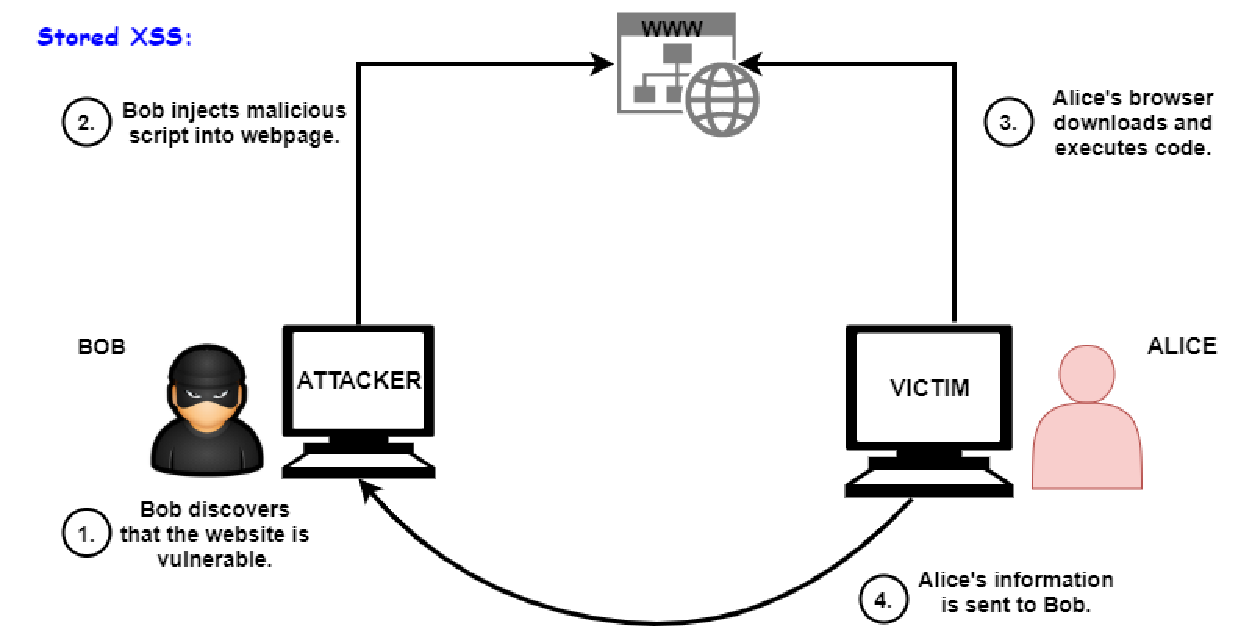
\includegraphics[width=\linewidth]{figures/storedxss.pdf}
 \caption{How Stored Cross-Site Scripting can be exploited by an attacker}
 \label{fig:storedxss}
\end{figure}

\begin{figure}[ht]
 \centering
 \captionsetup{justification=centering}
 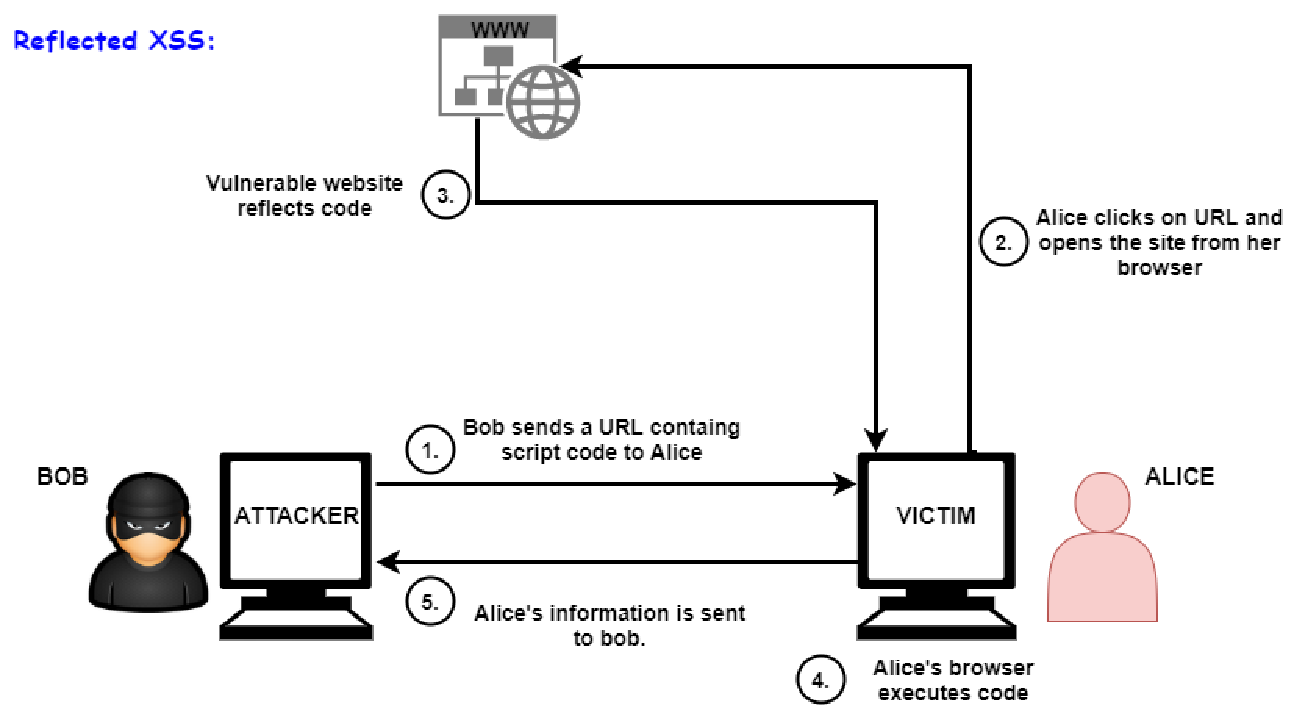
\includegraphics[width=\linewidth]{figures/reflectedxss.pdf}
 \caption{How Reflected Cross-Site Scripting can be exploited by an attacker}
 \label{fig:reflectedxss}
\end{figure}


The code above is faulty for two reasons. First, knowing a username exists offers clues for an attacker to guess a set of correct credentials much faster, since only the password is left to find. But this design choice is not linked with Cross-Site Scripting. The source of the bug is on line 11 where the error message "the \$username was not found" is displayed. Because {\tt \$username} is a tainted variable that has not been sanitized, an attacker can inject malicious payload in this field which will be interpreted by the HTML parser according to whatever its content is. 
{\tt Exploit:} A victim is tricked into submitting a form located in an attacker-controlled website. 

This malicious form is designed to trigger the vulnerability found in the above login form. As soon as the form is submitted the vulnerable login page is opened with the XSS script executed in it. If the victim now tries to login, the XSS script can easily send the
credentials to the attacker as well. 

Defeating XSS attacks is not dissimilar to defending against other types of code injection.
The input must be sanitized. User input containing HTTP code needs to be escaped or encoded to avoid its execution. Also, systemwide measures
such as Content Security Policy(CSP) ~\cite{csp_def} may be enabled to eliminate or mitigate XSS attacks. Nevertheless, flaws such as Buffer Overflows or Cross-Site Scripting issues comprise a majority of security incidents, and malicious hackers abuse them on a daily basis. 

\section{Fuzzing}
A promising method for discovering unknown vulnerabilities in
programs and web applications proven to be very effective, is a technique called fuzzing (or fuzz testing) ~\cite{fuzzing_def}. The technique was developed by Barton Miller et al. at the University of Wisconsin.
With this quality assurance technique, software is exercised using a vast number of anomalous inputs for inferring if any of them introduces security-related side effects. A fuzzer, which is the tool that can automate the aforementioned stress-testing process, can be categorized in relation to its awareness of the program structure as black-, white-, or gray-box ~\cite{fuzzing_book}. 

A black-box fuzzer treats the program as a black box and is unaware of
internal program structure. It conducts its test on the target through external
interfaces and produces random inputs using no information of the target's underlying structure. Hence,  black-box fuzzers are only able to scratch the surface usually and expose "shallow" bugs ~\cite{fuzzing_owasp}. 

A white-box fuzzer infers source code knowledge, such as source code auditing, to reveal
flaws in the software. It leverages program analysis to systematically
increase code coverage or to reach certain critical program locations. Program analysis can be based on either static or dynamic analysis, or their combination ~\cite{program_analysis_book}. They may also leverage symbolic execution in order to derive what inputs cause each part of a program to execute ~\cite{symbolic_exe}. Therefore, they can be very effective at exposing bugs that hide deep in the program. By studying the application code, you may be able to detect optional or proprietary features, which should be tested as well.

A fuzzer is considered gray-box when it leverages instrumentation rather than program analysis to glean information about the coverage of a generated input from the program it tries to fuzz ~\cite{zalewski2015american,efs2007}. This thesis explores in detail gray-box fuzzing, which is a combination of both the white-box and black-box approaches since it uses the internals of the software at a certain extend to assist in generating better test cases but still does not have full access to the code. Also the feasibility for constructing a fuzzing tool that will automate the process of discovering bugs in web applications is explored. This is succeeded by providing randomized invalid inputs to an under-analysis instrumented web application, mutating these inputs according to the feedback received and finding test cases that cause a crash or make them act inappropriately to better ensure the absence of exploitable vulnerabilities.

\section{Instrumentation}
Typically, a fuzzer is considered more effective if it achieves a higher degree of code coverage. This can be explained by the fact that to be able to trigger any given bug, the fuzzer must first execute the code where the bug lies. So widening code coverage increases the chances of executing unsafe pieces of code where bugs may reside. As mentioned in the previous section, using instrumentation may be the key to achieving a higher code-coverage percentage. 

However, some studies have failed to reach a consensus about the correlation between code coverage and the number of bugs found ~\cite{klees2018Evaluation,coverage2014effectiveness}. 
Increasing global code coverage may be less effective in finding new bugs than, for instance, focusing on widening code coverage in targeted error prone code areas as AFLGo ~\cite{bohme2017directed} does. Therefore code coverage should be considered a secondary metric and the number of bugs found as primary ~\cite{klees2018Evaluation}. Nevertheless, measuring coverage is important for any fuzzer.

Currently, available fuzzers for web applications act in a black-box fashion~\cite{doupe2010johnny}; they just use brute force at the target with URLs that embed known web-attack payloads with little or no information about the underlying structure of the target. 
In contrast, \pname firstly instruments a web application by adding code that tracks all control flows triggered by an input and notifies the fuzzer, accordingly. Notifications can be embedded in the web application's HTTP response using custom headers or it can be outputted to a shared file or memory region. 

On the other hand, the fuzzer starts sending requests to the target and analyses the responses to detect any requests of interest that would later help to improve the code coverage and as a result, trigger vulnerabilities nested deep in the web application's code. To calculate code coverage we simply calculate the ratio of how many basic blocks were visited in respect to the total number of basic blocks instrumented. This gives us a good idea of the coverage but omits crucial informations such as combinations of basic blocks that were visited one after the other.

We instrument web applications for delivering feedback once
they are fuzzed. As opposed to native applications, where
several options exist for instrumenting their source or binary
representation, we decide to instrument web applications by
modifying the Abstract Syntax Tree (AST) of PHP files and then reverting it back to source code form. This, in turn, provides us feedback on the basic blocks that are visited during analysis. For altering the AST of PHP files, PHP-Parser ~\cite{nikicPhpParser} is used. 
Instrumentation performed by \pname on our targeted web application is similar to how AFL instruments binaries, but adapted to work in web applications. A more elaborate approach of the instrumenting functionality provided by \pname is beyond the scopes of this thesis.

\section{Concurrency}
Concurrency is defined as working on multiple tasks at the same time ~\cite{concurrency_realpython}. However, in Python this does not mean that they work in parallel, since only one core of the CPU is active at any given time. Instead, each task takes turns in occupying the core and executing their code. When a task is interrupted, the state of each task is stored, so it can be restarted right from the point where it left off. 

Concurrency aims to speed up the overall performance of input/output (I/O) bound problems, whose performance can be slowed down dramatically when they are obliged to wait often for I/O operation from some external resource. An example of such a resource are requests on the internet or any kind of network traffic that can take several orders of magnitude longer than CPU instructions. An illustration of the above can be seen at Figure ~\ref{fig:concurrency_example}:

\begin{figure}[ht]
 \centering
 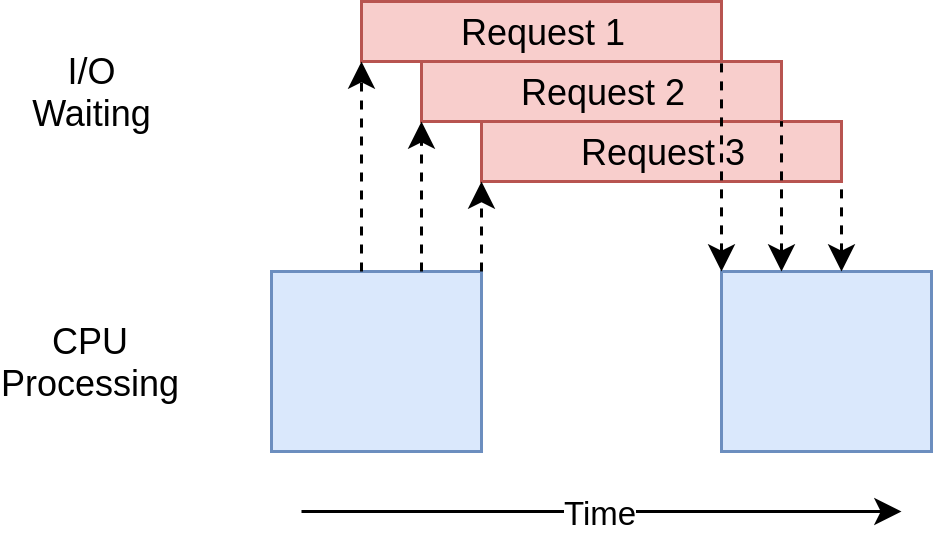
\includegraphics[width=\linewidth]{figures/concurrency_example.png}
 \caption{Requests over the internet processed in concurrent fashion ~\cite{concurrency_realpython}.}
 \label{fig:concurrency_example}
\end{figure}

More specifically in Python, concurrency can be expressed either through the Threading or AsyncIO(short for Asynchronous Input Output) ~\cite{asyncio} modules. Due to the infamous Global Interpreter Lock (GIL) ~\cite{gil_realpython} Python has, both AsyncIO and Threading are single-threaded, single-process design. Thus, there was no clear advantage of using the latter so AsyncIO was opted for instead, although the initial plan was to use threading. Not to mention the added complexity of using threads and making the program thread-safe. Briefly, GIL ensures there is only one thread running at any given time, thus making the use of multiple cores/processors with threads infeasible. 
In the Python community there is a general rule of thumb when it comes to I/O-bound problems; “Use asyncio when you can, threading when you must”.
More info on the AsyncIO module and its use in the \pname implementation can be found in Chapter ~\ref{sec:implementation}.

\section{Docker}
Docker containers ~\cite{docker_containers} provide developers the commodity of creating software locally with the knowledge that it will run identically regardless of the host environment ~\cite{using_docker_book}. Containers are an encapsulation of an application's dependencies that share resources with the host OS, unlike Virtual Machines. During the evaluation, which can be seen detailed in Chapter ~\ref{sec:evaluation}, a docker-compose YAML file was created to allow multiple containers to be initiated and managed at once with a set of pre-defined configurations. 

Services are deployed with containers through the use of Docker images. A Docker image consists of a collection of files that bundle together all the essentials, such as installations, application code and dependencies, required to configure a fully operational container environment. Official Docker images can be found at Docker Hub ~\cite{docker_hub}.